\chapter{Numerical Solution to Stochastic Burgers' equation}
\label{Chapter_4}
	
	In this chapter, we will study a spectral method to solve the Burgers' stochastic equation given by (\ref {burgers_stochastic2}). In the previous chapters we focus on spectral methods based on trigonometric polynomials to build a base on space, now in this method that we will present below, it will be constructed from another family of polynomials called Hermite polynomials. First, in the first two sections, we will study the theoretical basis of the method and its implementation. In the third section, the Burgers' stochastic equation method will be implemented. Finally, in the final section, we will present some important results of the numerical analysis of the method.\\
		
\section{Elemental Theory to Numerical Method}

	In statistical mechanics, the Fokker-Planck-Kolmogorov (FPK) equation is a partial differential equation that describes the temporal evolution of the probability density function of the velocity of a particle under the influence of drag forces and random forces, as in Brownian motion. The equation applies to systems that can be modified by a small number of "macrovariables", where other parameters can be quickly modified over time that can be treated as "noise" or a disturbance. The main idea is to associate the equation (FPK) with one (SPDE) through a stochastic differential equation. To do this, let's define the following. \\
	
	Set a separable infinite-dimensional Hilbert space $\mathcal{H}$ with inner product $\langle \cdot , \cdot \rangle_{\mathcal{H}}$. We define a Gaussian measure $\mu$ with mean zero and nuclear covariance operator $\Lambda$ with $Tr(\Lambda) < +\infty$. Setting the following stochastic differential equation in $\mathcal{H}$
   	\begin{align}
    	dX_t = AX_t dt + B(X_t) dt + \sqrt{Q} dW_t
    	\label{stochastic_equation}
   	\end{align}
   	where the operator $A : D(A) \subset \mathcal{H} \rightarrow \mathcal{H}$ is the infinitesimal generator of a strongly continuous semigroup $e^{tA} \in \mathcal{H}$, $Q$ is a bounded operator from another Hilbert space $U$ to $\mathcal{H}$ and $B : D(B) \subset \mathcal{H} \rightarrow \mathcal{H}$ is a nonlinear mapping.\\
   	
   	\noindent We define the next function
   	\begin{align}
   		u(x, t) = \mathbb{E} \left[ u_0 (X^x_t) \right] 
   		\label{solution_kolmogorov}
   	\end{align}
   	where $u_0 : \mathcal{H} \rightarrow \mathbb{R}$ and $X_t^x$ is the solution to (\ref{stochastic_equation}) with initial conditions $X_0 = x \in \mathcal{H}$. Then 
   	the equation (\ref{stochastic_equation}) can be associated with the Kolmogorov equation as following
   	\begin{align}
   		\label{kolmogorov}
    	\frac{\partial u}{\partial t} = \frac{1}{2} Tr(QD^2 u) + \langle Ax, Du\rangle_{\mathcal{H}} + \langle B(x), Du\rangle_{\mathcal{H}}, \hspace{0.1cm} x \in D(A)
   	\end{align}
   	where $u$ defined in (\ref{solution_kolmogorov}) satisfies (\ref{kolmogorov}). \\
   	 
   	\noindent Suppose that the operators $-A$ and $Q$ have the same eigenfunctions $e_k$ with eigenvalues $\lambda_k$ and $\rho_k$ respectively. We define the operator $\mathcal{L}$ as
   	\begin{align}
   	\label{operator_L}
   		\mathcal{L} u = \frac{1}{2} Tr(QD^2 u) + \langle Ax, Du\rangle_{\mathcal{H}}, \hspace{2mm} x \in \mathcal{H}
   	\end{align}
   	the operator $\mathcal{L}$ given above satisfies the following result.
   	\begin{lemma}
   	\label{eigen}
   		Let $H_n (h)$ be a Hermite polynomial functional given by (\ref{hermite_funcionals}). Then
   		the following holds: First, define $\mathcal{J}$ as follows
   		\begin{align*}
   			\mathcal{J} = \{\alpha = (\alpha_i,i \geq 1) | \alpha_i \in \mathbb{N}\cup \{0\}, |\alpha|:= \displaystyle \sum _{i = 0}^{\infty}\alpha_i < \infty\},
   		\end{align*}
   		hence
   		\begin{align}
   			\label{eigen_lambda_kolmo}
   			\mathcal{L} H_n (h) = - \lambda_n H_n (h)
   		\end{align}
   		for any $n \in \mathcal{J}$ and $H_n \in \mathcal{H}$, where
   		\begin{align*}
   			\lambda_n = \displaystyle \sum_{k=1}^{\infty} n_k \lambda_k
   		\end{align*}
   	\end{lemma}
   
   Using Lemmas \ref{dense} and \ref{eigen}, we have that $\{H_n \}$ forms a complete orthonormal system at $\mathbb{H}$. Therefore, if $u \in S(\mathbb{H})$ then 
   \begin{align}
   	\label{infinite_approximation}
   		u(x, t) = \displaystyle \sum_{n \in J} u_n (t) H_n (x), \hspace{2mm} x \in \mathcal{H}, \hspace{2mm} t \in [0, T],
   \end{align}
   
   where $u_n : [0, T] \rightarrow \mathbb{R}$ and $H_n (x)$ are the Hermite functionals. 
   
   \noindent Substituting (\ref{infinite_approximation}) into the equation (\ref{kolmogorov}) in the left side we get 
    \begin{align}
    \label{aprox_time}
    	\frac{\partial u}{\partial t} = \displaystyle \sum_{n \in J}  \dot{u}_n (t) H_n (x),
    \end{align} 
    the two first terms of the right side are obtained as
    \begin{align*}
    	\mathcal{L} u &= \mathcal{L} \left( \displaystyle \sum_{n \in J} u_n (t) H_n (x) \right) \\
    	&= \sum_{n \in J} u_n (t) \mathcal{L} H_n (x),
    \end{align*}
    and by Lemma \ref{eigen} we have
    \begin{align}
    \label{aprox_J}
    	\mathcal{L} u = - \sum_{n \in J} u_n (t) \lambda_n H_n (x).
    \end{align}	
    The last term of the equation is obtained as following
    \begin{align*}
    	\langle B(x), Du\rangle_{\mathcal{H}} = \left( B(x), D_x \displaystyle \sum_{n \in J} u_n (t) H_n (x)  \right)_{\mathcal{H}} 
    \end{align*}	
    \begin{align}
    \label{aprox_B}
    	\hspace{8mm} = \displaystyle \sum_{n \in J} u_n (t) \left( B(x), D_x H_n (x) \right)_{\mathcal{H}}
    \end{align}
    where $D_x$ denoting the Frechet Derivative. Therefore, by (\ref{aprox_time}-\ref{aprox_B}) the Kolmogorov equation becomes
    \begin{align*}
    	 \displaystyle \sum_{n \in J}  \dot{u}_n (t) H_n (x) = - \sum_{n \in J} u_n (t) \lambda_n H_n (x) + \sum_{n \in J} u_n (t) \left( B(x), D_x H_n (x) \right)_{\mathcal{H}}
    \end{align*}
    Multiplying the above equation by $H_m (x)$, $m \in J$ and integrating over $\mathcal{H}$ w.r.t. $\mu(dx)$ we have
    \begin{align*}
    	\displaystyle \sum_{n \in J}  \dot{u}_n (t) \int_{\mathcal{H}} H_m (x) H_n (x) \mu (dx) = &- \sum_{n \in J} u_n (t) \lambda_n \int_{\mathcal{H}} H_m (x)  H_n (x) \mu (dx) \\
    	&+ \sum_{n \in J} u_n (t) \int_{\mathcal{H}} H_m (x) \left( B(x), D_x H_n (x) \right)_{\mathcal{H}} \mu (dx)
    \end{align*}
    From the above and using the orthogonality of the system $\{H_m (x) \}$, we get a infinite system of coupled ordinary differential equations
    \begin{align}
    \label{infinite_system}
        \dot{u}_{m} (t) = -u_{m} (t) \lambda_{m} + \displaystyle \sum _{n \in \mathcal{J}} u_{n} (t) C_{n, m} , \hspace{2mm} n, m \in \mathcal{J}	
    \end{align}
    where $C_{n, m}$ is given by
    \begin{align}
    \label{Cnm}
    	C_{n, m} = \displaystyle  \int_{\mathcal{H}} H_m (x) \left( B(x), D_x H_n (x) \right)_{\mathcal{H}} \mu (dx)
    \end{align}
    
    \noindent Existence and uniqueness to above equation has been proven in \cite{Delgado2016}.
    
    \section{Numerical Approximation and Its Description}
    Define the set of finite multi-index $J^{M, N}$ as
    	\begin{align}
    		J^{M, N} = \{\gamma = (\gamma_i, \hspace{1mm} 1 \geq \gamma_i \geq M  ) \hspace{1mm} | \hspace{1mm} \gamma_i \in \{0, 1, \cdots, N \} \}
    	\end{align}
    this is the set of $M$-tuple which can take values in the set	$\{0, 1, \cdots, N \}$.\\
    
    \noindent The Approximation of the solution to equation (\ref{kolmogorov}) by (\ref{infinite_approximation}) is as following 
    \begin{align}
    \label{finite_approximation}
    	\hat{u}_N (x, t) = \displaystyle \sum_{ n \in J^{M, N} } u_n (t) H_n (x), \hspace{2mm} x \in \mathcal{H}, \hspace{2mm}, t \in [0, T].
    \end{align}
    
     \noindent Consider the same value $M$ as in $J^{M, N}$ and $m_1, m_2, \cdots, m_M \in J^{M, N}$. We define the finite system of equations, which is truncated the infinite system given by (\ref{infinite_system}).
    \begin{align}
    \label{finite_system}
    	\dot{u}_{m_i} (t) = -u_{m_i} (t) \lambda_{m_i} + \displaystyle \sum_{j=1}^{M} u_{n_j} (t) C_{n_j, m_i} , \hspace{2mm} 1 \geq i \geq M	
    \end{align}
    rewrite the above system in vectorial form as
    \begin{equation*}
    	U^M (t) =
    	\begin{pmatrix}
    		u_{m_1} (t) & u_{m_2} (t) & \dots & u_{m_M} (t)
    	\end{pmatrix}^T   
    \end{equation*}
    \begin{equation*}
    	\dot{U}^M (t) =
    	\begin{pmatrix}
    		\dot{u}_{m_1} (t) & \dot{u}_{m_2} (t) & \dots & \dot{u}_{m_M} (t)
    	\end{pmatrix}^T   
    \end{equation*}
   and the matrix $A$ is given by
    \begin{equation*}
   		A =
   		\begin{pmatrix}
	    	-\lambda_1 + C_{1,1} & C_{2,1} & \dots & C_{M-1,1} & C_{M,1} 
		    \\
		    C_{1,2} & -\lambda_2 + C_{2,2} & \dots & C_{M-1,2} & C_{M,2}  
		    \\
		    \vdots & \vdots & \ddots & \vdots & \vdots
		    \\
		    C_{1,M-1} & C_{2,M-1} & \dots & -\lambda_{M-1} + C_{M-1,M-1} & C_{M,M-1} 
		    \\
		    C_{1,M} & C_{2,M} & \dots & C_{M-1,M} & -\lambda_{M} + C_{M,M} 
	    \end{pmatrix}
    \end{equation*}
    where $\lambda_i = \lambda_{mi}$ and $C_{i, j} = C_{n_i, m_j}$ para $1 \leq i, j \leq M$. Notice that, given the
    expression (\ref{Cnm}), in general the matrix $A$ is not symmetric. We can now write the system (\ref{finite_system}) as a matrix differential equation:
    \begin{align}
    	\label{finite_system_vectorial}
    	\dot{U}^M (t) = AU^M (t)
    \end{align}
    
    \noindent Then, if $A$ has $M$ real and distint eigenvalues $\eta_i$ and $M$ eigenvectors $V_i$, then the solution to (\ref{finite_system_vectorial}) is given by
    \begin{align}
    \label{solution_finite_system}
    	 U^M (t) = \displaystyle \sum _{j = 1}^{M} c_i V_i e^{\eta_i t}
    \end{align}
    
    \noindent In the case when some of the eigenvalues and eigenvectors, or at least one of them, take values in the complex field we can still have real solutions. Indeed, suppose that we have the case with one complex eigenvalue and eigenvector then it is known that we will have $M - 2$ real eigenvalues but we can obtain two real solutions from the complex eigenvalue. \\
    
    \noindent Let us write one of the complex eigenvalues and eigenvectors as
    \begin{align*}
    	V &= a + i b \\
    	\eta &= \beta + i \mu
    \end{align*}
    then we can write two real solutions as follows:
    \begin{align*}
    	e^{\beta t} (a \cos(\mu t) - b \sin(\mu t)), \hspace{2mm} e^{\beta t} (a \sin(\mu t) + b \cos(\mu t))
    \end{align*}
    
    \subsection{Initial Conditions}
    
    In contrast to several types of differential equations, whether ordinary or partial, deterministic or stochastic, for FPK equations there is no standard way to determine the initial conditions. This is because in this type of equations we must choose a functional that acts on the initial condition, this implies that depending on the functional chosen we must adapt the method. \\
    
    \noindent Here we present the method for two examples of functionals, but only one be devoloped. We will consider two cases:
    \begin{align*}
    	u^{z_0}_0 (g) := g(z_0), \hspace{2mm} \text{for fixed} \hspace{2mm} z_0 \in [0, 1].
    \end{align*}
    \begin{align*}
    	u_0 (g) := \displaystyle \int_{0}^{1} g(z) dz.
    \end{align*}
    
    \noindent For the first functional, define the set points into the set $[0, 1]$ as 
    \begin{align*}
    	P = \{ z_i, \hspace{1mm} 0 \leq i \leq p \hspace{1mm} : \hspace{1mm} z_0 = 0, \hspace{1mm} z_p = 1 \}
    \end{align*}
    
    \noindent Then for each point $z_i \in P$ such that $X_0 (z_i) = X(0, z_i)$ set $u_0 (x)$ as the evaluation functional $z_i \longrightarrow X^x_t (z_i)$. Then from (\ref{solution_kolmogorov}) we obtain
    \begin{align}
   		u(0, x) = \mathbb{E}[u^{z_i}_0 (X^x_0)] = X^x (0, z_i) = x(z_i)
    \end{align}
    For other hand
    \begin{align*}
    	u (0, x) = \displaystyle \sum _{n \in \mathcal{J}^{M, N}} u_{n}(0) H_n (x)
    \end{align*}
    multiplying for $H_m (x)$ and integrating over space $\mathcal{L}^2 (\mathcal{H}, \mu)$ 
    \begin{align*}
    	u_m (0) = \displaystyle \int_{\mathcal{H}} x(z_i) H_m (x) \mu (dx)
    \end{align*}
    
    \noindent Note that in the direction of the eigenfunction $e_k$ the expression $x$ can be written as $(x, e_k )_{\mathcal{H}} e_k$, then we can write $H_m (x) x (z_i)$ in the direction $e_k$ as $P_{m_k} (\xi_k) (x, e_k )_{\mathcal{H}} e_k (z_i)$ with $\xi_k = (x, \Lambda^{-\frac{1}{2}} e_k) = \| \lambda_k \| (x, e_k )_{\mathcal{H}}$ and $P_{m_k}$ is given by (\ref{hermite_polynomials}). Then we have
    \begin{align*}
    	u^{z_i}_m (0) &= \displaystyle \int_{\mathcal{H}} x(z_i) H_m (x) \mu (dx) \\
    	&= \int_{\mathbb{R}^N} \sum_{k=1}^{\infty} P_{m_k} (\xi_k) (x, e_k )_{\mathcal{H}} e_k (z_i) \mu (d\xi_1, d\xi_2, \cdots) e_k \\
    	&= \int_{\mathbb{R}^N} \sum_{k=1}^{\infty} P_{m_k} (\xi_k) \frac{\xi_k}{\lambda_k} e_k (z_i) \mu (d\xi_1, d\xi_2, \cdots) e_k \\
    	&= \sum_{k=1}^{\infty} \frac{e_k}{\lambda_k} \int_{\mathbb{R}}  P_{m_k} (\xi_k) \xi_k (z_i) \mu (d\xi_k)
    \end{align*}
    truncating the above expression we have
    \begin{align}
    \label{IC_approx}
    	u^{z_i}_m (0) \approx \displaystyle \sum_{k=1}^{M} \frac{e_k}{\lambda_k} \int_{\mathbb{R}}  P_{m_k} (\xi_k) \xi_k (z_i) \mu (d\xi_k)
    \end{align} 
    
    \noindent Setting the equation (\ref{IC_approx}) for each element from $u^{z_i}_m$ as $u^{z_i}_{m_j} (0) = u_j (0)$, $1 \leq j \leq M$ and by (\ref{solution_finite_system}) evaluated for $t=0$, then the initial condition can be written as
    \begin{equation*}	
	    \begin{pmatrix}
	    u_1 (0) \\ u_2 (0) \\ \vdots \\ u_{M-1} (0) \\	u_M (0)
	    \end{pmatrix}
	    = 
	    \begin{pmatrix}
	    V1 & V2 & \dots & V_{M-1} & V_M
	    \end{pmatrix}
	    \begin{pmatrix}
	    c_1 \\ c_2 \\ \vdots \\ c_{M-1} \\ c_M
	    \end{pmatrix}
    \end{equation*}
    and the constants $c_j$ are calculated as
    \begin{equation*}
    	\begin{pmatrix}
    	c_1 \\ c_2 \\ \vdots \\ c_{M-1} \\ c_M 
    	\end{pmatrix}
    	=	
    	\begin{pmatrix}
    	V1 & V2 & \dots & V_{M-1} & V_M
    	\end{pmatrix}^{-1}
	    \begin{pmatrix}
	    u_1 (0) \\ u_2 (0) \\ \vdots \\ u_{M-1} (0) \\	u_M (0)
	    \end{pmatrix}
    \end{equation*}
    
    \section{Numerical Approximation to Stochastic Burgers' Equation}
    Let $\mathcal{H} = L^2 (0, 1)$. We consider the problem given by (\ref{burgers_stochastic}) over the interval $[0, 1]$ ,
	\begin{align}
		\label{burgers_stochastic2}
		d X(\xi, t) = \left[\alpha \partial_{\xi}^2 X(\xi, t) + \frac{1}{2} \partial_\xi \left(X^2 (\xi, t)\right) \right] dt + dW_t (\xi, t), \hspace{0.2cm} \xi \in [0, 1] 
	\end{align}
	The boundary condition and its initial condition are respectively 
	\begin{align*}
		%\label{IC_burgers_stochastic2}
    	X(0, t) &= X(1, t) = 0 , \hspace{0.2cm} t > 0 \\
		X(\xi, 0) &= x(\xi), \hspace{0.2cm}  x \in \mathcal{H},
	\end{align*}
	where $W$ is a cylindrical Wiener process on $\mathcal{H}$ as was given by \ref{cylindrical}, associated to a stochastic basis $(\Omega, \mathcal{F}, \mathbb{P}, \{\mathcal{F}_t\}_{t \geq 0})$, and as usually $\alpha > 0$ is the viscosity coefficient. \\

	\noindent Setting $A = \alpha \partial^2_{\xi}$ and $B = \frac{1}{2} \partial_{\xi} (x^2)$, $x \in \mathcal{H}$, with its domains $D(A) = H^2 (0, 1) \cap H^1_0 (0, 1)$ and $D(B) = H^1_0 (0, 1)$ respectively, then by (\ref{stochastic_equation}), with $Q = Id$, the equation (\ref{burgers_stochastic2}) can be rewritten as
	\begin{align*}
    	dX &= [AX + B(X)]dt + dW_t \\
        X(0) &= x, \hspace{0.2cm} x \in \mathcal{H}
	\end{align*}	
	As we know the operator $A$ is a infinitesimal generator of a strongly continuous semigroup $e^{At}$ in $\mathcal{H}$, also is self-adjoint that has a complete orthonormal system of eigenfunctions in $\mathcal{H}$ given by
	\begin{align*}
		e_k (\xi) = \sqrt{2} \sin{(k \pi \xi)}, \hspace{3mm} \xi \in [0, 1], \hspace{3mm} k \in \mathbb{N}
	\end{align*}
	
	\noindent Note that the operator $A$ satisfies $Ae_k = -\alpha \pi^2 k^2 e_k$ for $k \in \mathbb{N}$, then if we set $\Lambda = (-A)^{-1}$ we have that $\Lambda^{-1/2} e_k = \sqrt{2 \alpha} \pi |k| e_k$. \\	
		
	\noindent If we define $u(x, t) \in S (\mathbb{H})$ as was defined by (\ref{solution_kolmogorov}), then $u$  satisfies Kolmogorov equation given by (\ref{kolmogorov}). So, the descomposition for $u \in S (\mathbb{H})$ given by (\ref{infinite_approximation}) gives 
	\begin{align}
		u(t, x) = \displaystyle \sum _{n \in \mathcal{J}} u_{n}(t) H_n (x), \hspace{0.1cm} x \in \mathcal{H}, \hspace{0.1cm} t \in [0, T],
	\end{align}		
	to get the following system as was given by (\ref{infinite_system})
	\begin{align}
		\dot{u}_{m} (t) = -u_{m} (t) \lambda_{m} + \displaystyle \sum _{n \in \mathcal{J}} u_{n} (t) C_{n, m} , \hspace{0.1cm} n, m \in \mathcal{J}
	\end{align}
		
	\noindent We need to calculate the value of the constants $C_{n,m}$ , then we need to calculate expressions such as $B(x)$, $D_x H_n (x)$. Note that $x$ can be written as $x = \displaystyle \sum_k \beta_k e_k$ , with $\beta_k := \langle x, e_k \rangle_{\mathcal{H}}$. Then we have
	\begin{align*}
		B(x) = \frac{1}{2} \partial_{\xi} \left( \displaystyle \sum_k \beta_k e_k \right)^2 = \frac{1}{2} \partial_{\xi} \left[ \sum_l
		\sum_k \beta_l \beta_k e_l e_k \right] = \frac{1}{2} \sum_l
		\sum_k \beta_l \beta_k (e_l e'_k + e'_l e_k)
	\end{align*}
	and for $D_x H_n (x)$ we have
	\begin{align*}
		D_x H_n (x) = \displaystyle \sum_{j = 1}^{\infty} \prod_{i = 1. i \neq j}^{\infty} P_{n_i} (\langle x, \Lambda^{-1 / 2} e_i \rangle_{\mathcal{H}}) P'_{n_j} (\langle x, \Lambda^{-1 / 2} e_j \rangle_{\mathcal{H}}) \Lambda^{-1 / 2} e_j 
	\end{align*}
	
	\noindent Therefore, $C_{n, m}$ given by (\ref{Cnm}) gives
	\begin{align*}
		C_{n, m} =& \displaystyle \frac{1}{2} \int_{\mathcal{H}} H_m (x) \mu (dx) \sum_{j = 1}^{\infty} \prod_{i = 1, i \neq j}^{\infty} P_{n_i} (\langle x, \Lambda^{-1 / 2} e_i \rangle_{\mathcal{H}}) P'_{n_j} (\langle x, \Lambda^{-1 / 2} e_j \rangle_{\mathcal{H}})  \sqrt{2 \alpha} \pi |j| \\
		&\cdot \sum_l
		\sum_k \beta_l \beta_k (e_l e'_k + e'_l e_k) \\
		=& \displaystyle \frac{1}{2} \int_{\mathcal{H}} \mu (dx) \sum_{j = 1}^{\infty} \sqrt{2 \alpha} \pi |j| P_{m_j} (\langle x, \Lambda^{-1 / 2} e_j \rangle_{\mathcal{H}}) P'_{n_j} (\langle x, \Lambda^{-1 / 2} e_j \rangle_{\mathcal{H}}) \\  &\cdot \prod_{i = 1, i \neq j}^{\infty} P_{n_i} (\langle x, \Lambda^{-1 / 2} e_i \rangle_{\mathcal{H}}) P_{m_i} (\langle x, \Lambda^{-1 / 2} e_i \rangle_{\mathcal{H}}) \\
		&\cdot \sum_l
		\sum_k \beta_l \beta_k (e_l e'_k + e'_l e_k) 
	\end{align*}
	For $N_1 \in \mathbb{N}$ define as before the set $S_{N_1} = \{n_1 , n_2 , \cdots , n_{N_1} : n_i \in J^{M,N} , i = 1, \cdots , N_1 \}$. Then for $n, m \in S_{N}$ we have 
	\begin{align*}
		\bar{C}_{n, m} =& \displaystyle \frac{1}{2} \sum_{j = 1}^{\infty} \sqrt{2 \alpha} \pi |j| \int_{\mathcal{\mathbb{R}^M}} P_{m_j} (\xi_j) P'_{n_j} (\xi_j) \mu (d \xi_j) \\  
		&\cdot \prod_{i = 1, i \neq j}^{M} P_{m_i} (\xi_i) P_{n_i} (\xi_i) \mu (d \xi_i) \sum_{l=1}^{M} \sum_{k=1}^{M} \beta_l \beta_k (e_l e'_k + e'_l e_k)
	\end{align*}
	 So, the finite system of ordinary differential equations has the following form
	\begin{align}
	\label{burgers_stochastic_aprox}
		\dot{u}_{m} (t) = -u_{m} (t) \lambda_{m} + \displaystyle \sum _{n \in S_N} u_{n} (t) \bar{C}_{n, m} , \hspace{0.1cm} n, m \in S_N
	\end{align}
	Therefore (\ref{burgers_stochastic_aprox}) approximates to the infinite system of ordinary differential equations (\ref{infinite_system}) when $N, M \rightarrow \infty$.
	
	\section{Something about Numerical Analysis}
    
    In this section, we will study some results of the numerical analysis of the method described above that have been studied in \cite{Delgado2019}. Something that we are going to observe is that the analysis is very similar to the deterministic case we saw in the previous chapter. \\
    
    \noindent Recall that the solution $u(x, t)$ for (\ref{kolmogorov}) is given by
    \begin{align*}
    	u(x, t) = \mathbb{E} \left[ \varphi (X^x_t) \right]. 
    \end{align*}
    where $\varphi: \mathcal{H} \rightarrow \mathbb{R}$ and $X^x_t$ is the solution to (\ref{stochastic_equation}) with initial conditions $X_0 = x \in \mathcal{H}$. Then by Lemma \ref{eigenvalues_lambda} we can written the solution $\psi^x_t$ as follows 
    \begin{align*}
    	\Psi^{\varphi}_t = \displaystyle \sum _{n \in \mathcal{J}} u_n (t) H_n (x), \hspace{2mm} x \in \mathcal{H}, \hspace{2mm} t \in [0, T].
    \end{align*}
	
	The following result show the continuity with respect to the initial conditions for a numerical approximation of the Kolmogorov equation associated with an SPDE. Here we understand that a numerical scheme is stable respect to initial conditions if this method reproduces the same behavior when the continuous problem satisfies continuity respect initial conditions.
	
	\begin{teor}
		Assume that the eigenvalues of $\Lambda$, satisfies that for every $k \in \mathbb{N}$, $\lambda_k < \lambda_{k+1} \rightarrow \infty$. Assume that the functional $\varphi$ is Lipschitz. Then, the nu-
		meric approximation $\Psi^{\varphi}_t$ to the solution of the Kolmogorov equation $\psi \in C((0, T), \mathbb{H})$ depends continuously on the initial conditions, i.e., for two different initial values $x, y \in \mathcal{H}$
		\begin{align*}
			\| \Psi^x_t - \Psi^y_t \|^2_{\left( L^2 (\mathcal{H}, \mu)\right)^2} \leq \exp(Ct) \displaystyle \int_{\mathcal{H} \times \mathcal{H}} \|x - y \|^2_{\mathcal{H}} \mu (dx) \mu (dy) + f(t) \|x - y\|_{\mathcal{H}},
		\end{align*}
		for some $C>0$ and $f(t)$ is given by
		\begin{align*}
			f(t) = \displaystyle \sum_{n \in J} \left[u^y_n (t)\right]^2 + \int_{\mathcal{H}} \mathbb{E}^2 \left[\varphi (X^y_t)\right] \mu (dy).
		\end{align*}	
		Equivalently, if $\|x - y\|_{\mathcal{H}} \leq \delta$ then
		\begin{align*}
			\| \Psi^x_t - \Psi^y_t \| \leq G(t) \delta.
		\end{align*} 
	\end{teor}
	
	\noindent For ilustrate the above Theorem, numerical experiments were performed using as initial condition $x(\xi)$ for equation (\ref{burgers_stochastic2}) and its truncated Chebyshev expansion with polynomials of the first kind given by
	\begin{align*}
		x(\xi) = \sin(\pi \xi), \hspace{3mm} y(\xi) = \displaystyle \sum^{N}_{k=0} c_k T_k (\xi),
	\end{align*}
	with a discretization of $2048$ points in spatial variable $\xi$ over $[0, 1]$, $1024$ points in time variable $t$ over $[0, 10]$, and with parameters $\alpha = 0.01$, $N = 5$, $M = 11$ for using approximation given by (\ref{burgers_stochastic_aprox}).
	
	\begin{figure}[H]
		\centering	
		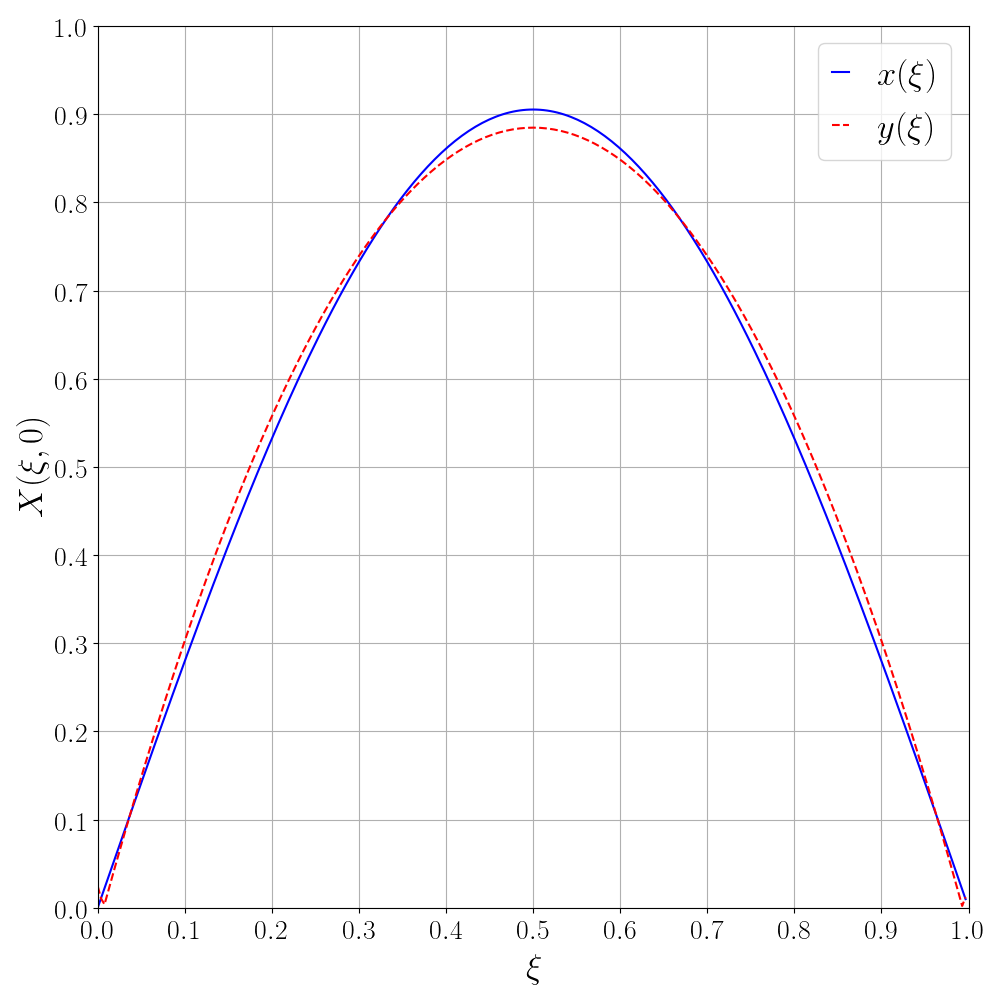
\includegraphics[width=.55\textwidth]{Figures/IC.png}
		\caption{Initial condition for (\ref{burgers_stochastic2}) and its approximation.}
		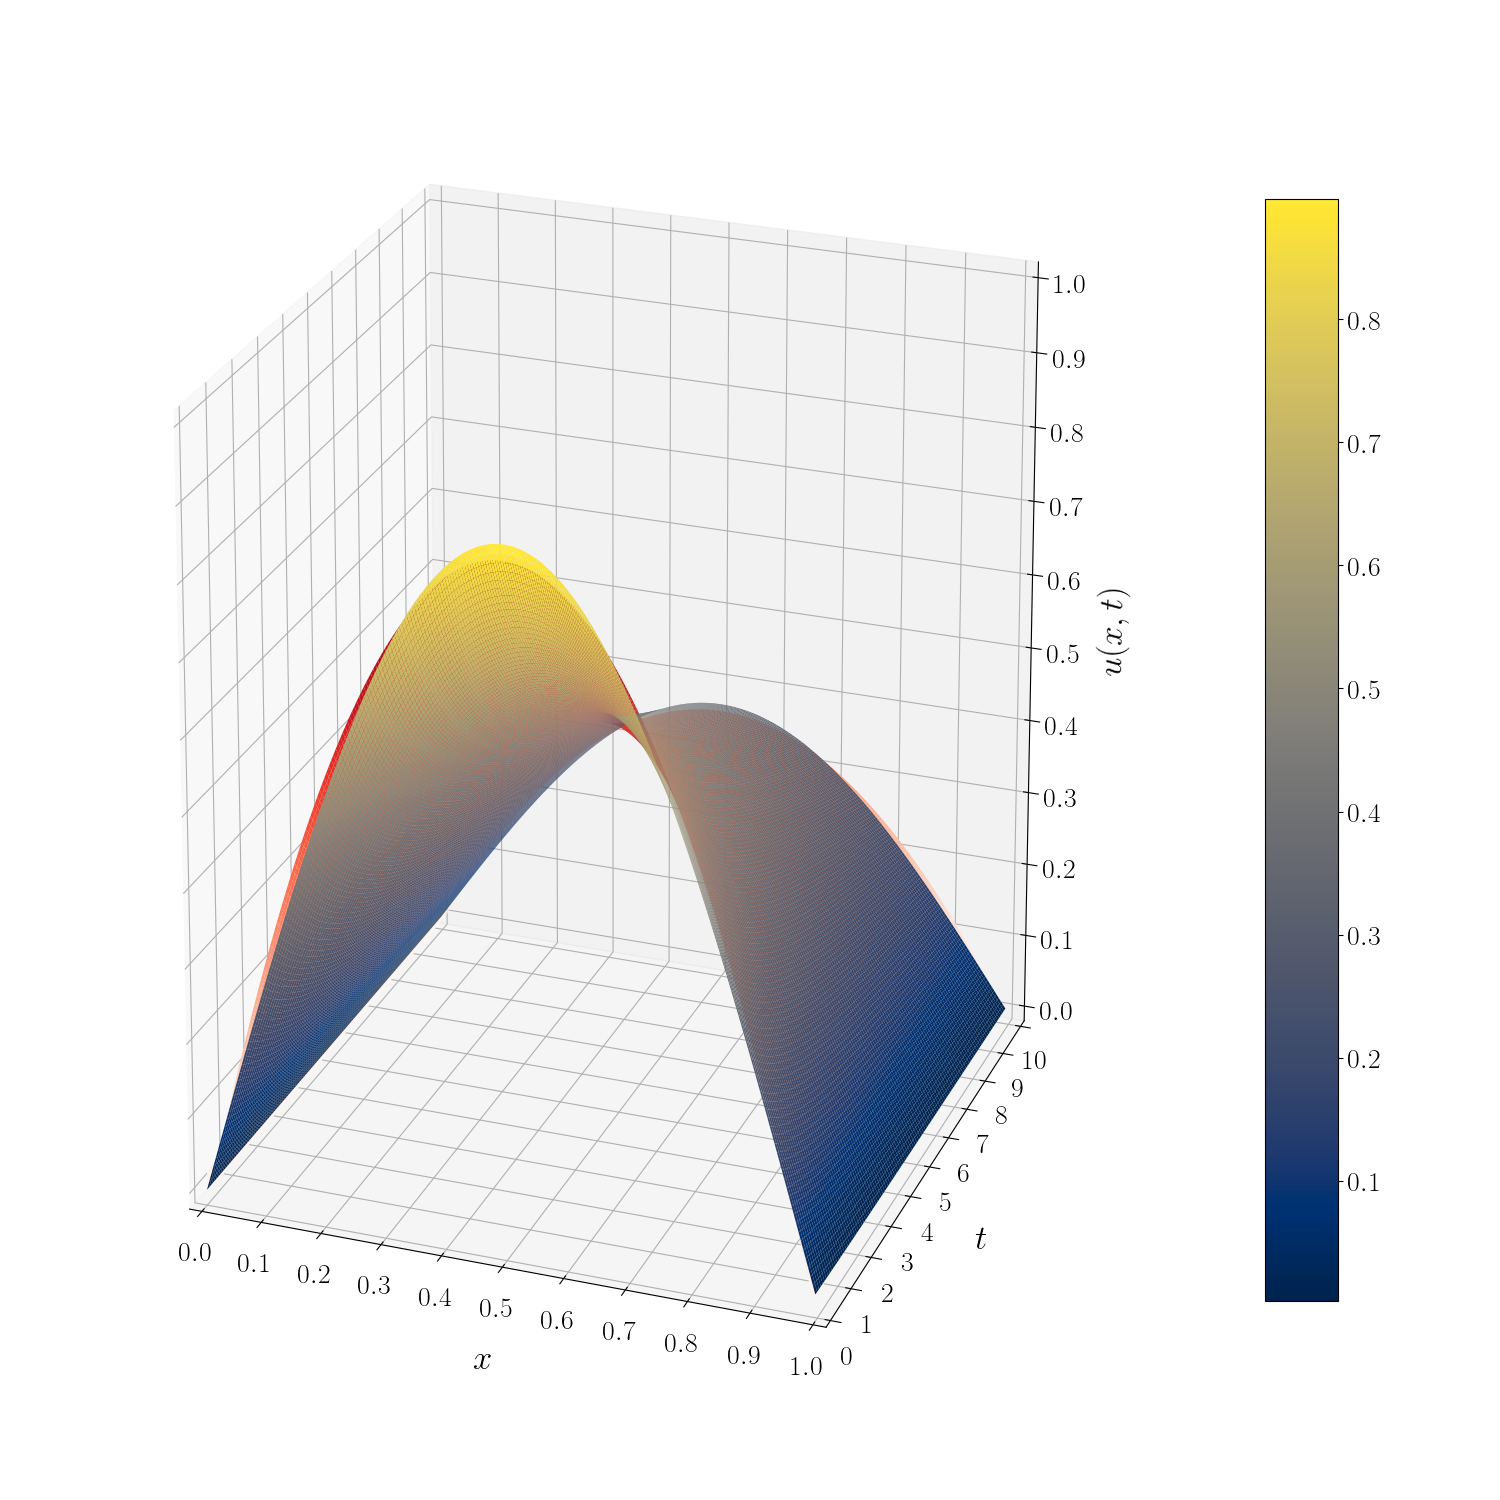
\includegraphics[width=.9\textwidth]{Figures/Numerical_Solution_Stochastic.png}
		\caption{Numerical solutions for (\ref{burgers_stochastic2}) with initial conditions $x(\xi)$ and $y(\xi)$.}
	\end{figure}
	
	\begin{figure}[H]
	\centering
		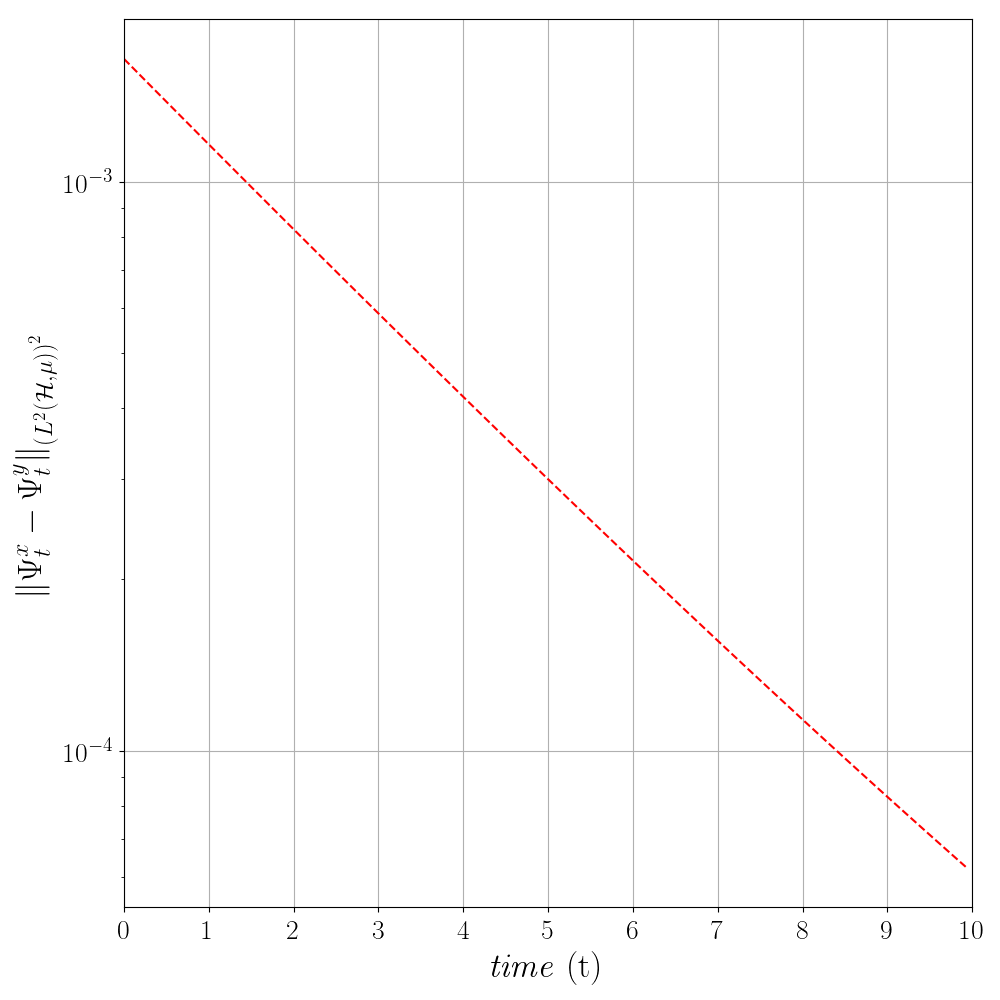
\includegraphics[width=.7\textwidth]{Figures/norms.png}
		\caption{Distance between the numerical solutions for equation (\ref{burgers_stochastic2}) with initial conditions $x(\xi)$, and $y(\xi)$.}
	\end{figure}
	
	The stability version presented above says merely that method preserve the continuity respect to initial conditions, i.e., if a given problem satisfies certain regularity conditions, then two of its solution remain closed if its initial function conditions are close. So, we desire that a numerical method reproduce this behavior and if it is the case, we say that an underlying method is stable in this context. However, the stability theory for spectral methods is still under construction and is an active research area. 
	
	%For instance, some works of L.N. Trefethen and M.R. Trummer [17], D. Gottlieb et. al. [12] as reference for the deterministic case, and N. Li, J. Fiordilino, and X. Feng, [15] A. Lang, A. Petersson, and A. Thalhammer, [14] for the stochastic version.  \\
	
	This kind of stability, combining with the weak approximation approach, would save computation time. Since the scheme asks specific conditions to obtain a weak numerical solution of an underlying SPDE, so convert the stochastic problem into a deterministic ODE for the first moment. This procedure overcome Montecarlo type simulations to approximate moments or distributions—simulate many realization of the numerical stochastic process to approximate distributions or moments.	 